\section{Managementprozess}

\textit{Bearbeitet von: Olga Miloevich}\\

\subsection{Managementprozess und --prioritäten}

\textit{Folgender Abschnitt w"urde von Projektplan von der Gruppe YNotZoidberg (Vorlesung Software Projekt 2, WiSe2013/14, S. 6-11 "ubernommen}\\

F"ur die Organisation unseres Projektes haben wir einen Projektleiter gew"ahlt.\\
Wir haben zudem die Gruppe in einzelne Arbeitsgruppen eingeteilt. Daf"ur haben wir nach einem schnellen dynamischen System aus der Wirtschaft gesucht und haben das sogenannte Mehrliniensystem ausgew"ahlt. Dieses Mehrliniensystem ist im Gegensatz zur Matrixorganisation oder dem Einzelliniensystem am besten f"ur unsere Umst"ande und Zwecke geeignet. Das System passt am besten f"ur kleine Gruppen, wie unsere. Es lassen sich mehrere Personen zu einer Gruppe zuordnen. \newline
Der Projektmanager "uberwacht den Ablauf des gesamten Projektes und kontrolliert die Arbeitsgruppen. Die Arbeitsgruppen kommunizieren mit den jeweiligen Mitgliedern ihrer Arbeitsgruppe sowie mit allen Gruppenleitern. Bei Bedarf kommunizieren die Arbeiter einer Arbeitsgruppe auch mit Arbeitern anderer Arbeitsgruppen. \\
Die Kommunikationen innerhalb der gesamten Projektgruppen wird durch regelm"a"sige Meetings gew"ahrleistet. Bei Konflikten oder Unstimmigkeiten ist der Projektleiter ein Ansprechpartner und auch Entscheidungstr"ager.\\
Unsere Priorit"ateten liegen bei diesem Projekt haupts"achlich bei der Erf"ullung der Mindestanforderunden in dem gegebenen Zeitraum. Dabei haben wir auch einen Puffer eingeplant. Werden die Mindestanforderunden fr"uhzeitig erf"ullt, dann wird dieser Puffer dazu benutzt, einige Zusatzfunktionen in unsere Software zu integrieren. \\
Unser Budget besteht aus Personen und Personenstunden. Die Planung dieses Budgets "ubernimmt der Projektleiter.\\
Es folgt unser Mehrliniendiagramm.\\
\textit{Quellen: Projektplan von der Gruppe ``Five and a half men'' (Vorlesung Software Projekt 1 2013); Projektplan von der Gruppe ``irgendwiecool'' (Vorlesung Software Projekt 2 2013); Projektplan von der Gruppe ``ICC'' (Vorlesung Software Projekt 1 2013);  Projektplan von der Gruppe ``YNotZoidberg'' (Vorlesung Software Projekt 2 2013/14)}
\newpage
\begin{figure}[h!]
\center{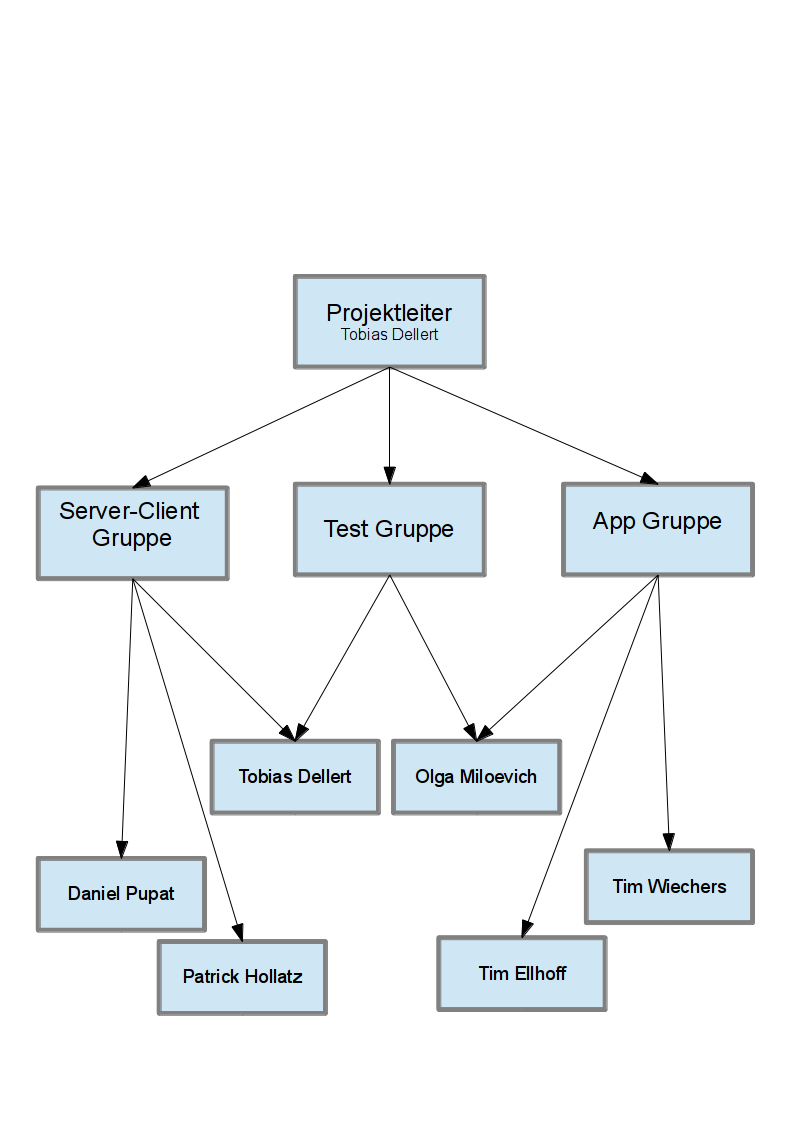
\includegraphics[scale=0.675]{MPGL.png}}
\caption{Mehrliniendiagramm}
\label{Bild:image}
\end{figure}


\subsection{Annahmen, Abhängigkeiten und Einschränkungen}

\textbf{Annahmen}
\begin{itemize}
 \item Jeder Mitarbeiter besitzt Kenntnisse in Java, Latex und SQL.
\end{itemize}

\textbf{Abhängigkeiten}
\begin{itemize}
 \item Es gibt festgelegte Deadlines.
 \item Der jetzige Zeitplan wird sich z.B. bei Personalausfall ändern.
\end{itemize}

\textbf{Einschränkungen}
\begin{itemize}
 \item Wir haben vorgegebene Technologien und Sprachen zu verwenden (Java, SQL etc.) 
 \item Der Zeitplan ist eingeschränkt, für jede Abgabe ist ein festes Datum gesetzt.

\end{itemize}

\subsection{Risikomanagement}\label{riskmanagement}
